\section*{Ergebnisse}
\label{sec:Ergebnisse}

Die Faktorenanalyse liefert vier Faktoren aus den 13 von Probanden bewerteten Attributen Anspruchsvoll, Einfach, Emotional, Entspannend, Erregend, Fröhlich, Intellektuell, Intensiv, Komplex, Sanft, Tanzbar, Traurig und Warm. 
Dabei wurde das Kaiser-Kriterium für signifikante Faktoren ab einem Eigenwert von mindestens 1 berücksichtigt.
Das Kaiser-Meyer-Olkin-Kriterium der Faktorenanalyse nimmt einen Wert von 0,734 an, was einem \textit{ziemlich guten} Ausmaß an Interkorrelation zwischen den Variablen entspricht \cite{eckey2002multivariate}.
Die vier Faktoren decken insgesamt 67\% der Gesamtvarianz.
Wenige Variablen laden dabei mit einer Faktorladung von mindestens 0,66 relativ stark in einen Faktor, während sie gleichzeitig mit einem maximalen Wert von 0,46 eher schwach in die übrigen Faktoren laden.
Einzig die Variable \textit{Emotional} lädt in keines der Faktoren stark und entfällt aus diesem Grund aus der inhaltlichen Beschreibung der erzeugten Faktoren.
Die vier erzeugten Faktoren werden inhaltlich gekennzeichnet als \textit{Ruhig} für den 1. Faktor, \textit{Niveauvoll} für den 2. Faktor, \textit{Heiter} für den 3. Faktor und \textit{Energisch} für den 4. Faktor (vgl. Tabelle \ref{tab:faktoren}).   


\begin{table}[htbp]
    \centering
    \caption{Faktoren}
    \vspace{2mm}
    \label{tab:faktoren}
        \begin{tabularx}{8cm}{|X|X|X|X|}
            \hline Faktor 1: Ruhig & Faktor 2: Niveauvoll & Faktor 3: Heiter & Faktor 4: Energisch \\
            \hline Entspan\-nend & Anspruchs\-voll       & Fröhlich             & Erregend \\
            \hline Warm              & Komplex                  & -Traurig             & Intensiv \\
            \hline Sanft               & - Einfach                 & Tanzbar             & \\
            \hline                        & Intellek\-tuell          &                          & \\
            \hline
        \end{tabularx}
\end{table}

Die Regressionen dieser Faktoren mit den Features von Spotify liefern Modelle mit hohen Signifikanzen. Abgesehen von der Regression mit dem Faktor \textit{Niveauvoll}, dass ein Modell mit einer Signifikanz von 0,017 erstellt, erhalten die Modelle mit den restlichen Regressionen Signifikanzen mit einem Wert von 0,000. 
Das Modell mit der höchsten Güte erhalten wir bei der Regression mit dem Faktor \textit{Heiter}.
Mit einem Wert von 0,231 für das Bestimmtheitsmaß wird 23,1\% der Varianz vom Modell, dass die Variablen \textit{SP\_danceability}, \textit{SP\_energy}, \textit{SP\_instrumentalness} und \textit{SP\_valence} enthält, gedeckt.
Die Variable \textit{SP\_energy} ist in dem Modell mit einem Beta Wert von 0,279 am stärksten gewichtet, gefolgt von den Variablen \textit{SP\_danceability} (0,247),  \textit{SP\_instrumentalness} (0,204) und \textit{SP\_valence} (0,136).
Das Streudiagramm dieser Regression ist in Abb. \ref{fig:Faktor3} zu sehen.    
Ein Modell mit einer ähnlich hohen Güte (0,215) gibt die Regression mit dem Faktor \textit{Ruhig} aus.
21,5\% der Varianz wird durch dieses Modell gedeckt.
Enthalten in diesem Modell ist die Variable \textit{SP\_energy}, die mit einer negativen Effektstärke mit einem Beta Wert -0,434 etwa vier mal stärker gewichtet ist als die zweite in dem Modell enthaltenen Variable \textit{SP\_speechiness} (-0,100).
Deutlich schlechtere Modellanpassungen leifert die Regressionen mit den Faktoren \textit{Niveauvoll} und \textit{Energisch}.
Wir erhalten ein Modell mit einer Güte von 0,112 bei der Regression mit dem Faktor \textit{Energisch} und nur 0,038 bei der Regression mit dem Faktor \textit{Niveauvoll}.


\begin{figure}[hbt]
    \begin{center}
        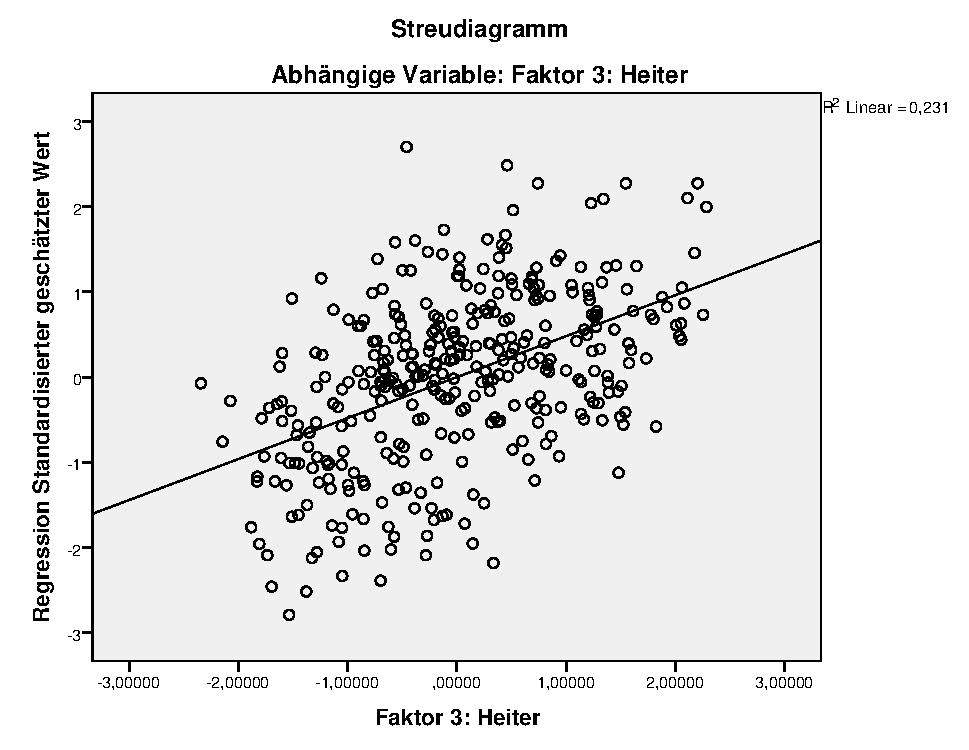
\includegraphics[width=8cm]{images/StreudiagrammFak3.pdf}
    \end{center}
    \caption{Streudiagramm und Regressionsgerade der Regression mit dem Faktor \textit{Heiter}.}
    \label{fig:Faktor3}
\end{figure}

\section*{Diskussion}
\label{sec:Diskussion}


Die Modelle der Regressionen sind hochsignifikant.
Somit ist ein Zusammenhang zwischen den Bewertungen der Probanden und den Features von Spotify vorhanden.
Die Effektstärken der Modelle sind dagegen eher gering.
Die in der Hypothese formulierte Annahme der starken Korrelation .... mit einem Wert von ??? kann somit nicht bestätigt werden.

Die eher schwachen Korrelationswerte der beiden Datensätze vermuten einen mangelhaften Algorithmus von Spotify zur Bewertung von Musikstücken.
Fehler müssen jedoch nicht nur bei den Spotify Algorithmen liegen.
Auch beim Datensatz ``10 Songs für die Insel'' sind Fehler zu erwarten.
Jeder Songs wurden jeweils nur einmal von nur einer Person bewertet.
Hinzu kommt, dass die Probanden einen besonderen, persönlichen Bezug zu den von ihnen bewerteten Musikstücken haben.
Mehrere Bewertungen eines einzelnen Musikstücks durch mehreren Probanden mit anschließender Mittelung würde zu einer Verringerung des Fehlers und aussagekräftigeren Ergebnissen führen.

Ein weiterer Grund für die geringe Korrelation könnte aber auch die inhaltlich meist nicht direkt entsprechenden Bewertungskriterien beider Datensätze sein.
Es gibt beispielsweise für den Faktor mit dem schwächsten Korrelationswert, \textit{Niveauvoll}, kein Spotify Feature, das diesem Faktor inhaltlich zuzuordnen werden könnte. 
Dahingegen lässt sich eine starke negative Korrelation des Spotify Features \textit{SP\_energy} mit dem Faktor \textit{Ruhig} inhaltlich sinnvoll erschließen.
Gleiches gilt auch für die Korrelation der Features \textit{SP\_danceability}, \textit{SP\_energy}, \textit{SP\_instrumentalness} und \textit{SP\_valence} mit dem Faktor \textit{Heiter}.
Die Spotify Features \textit{SP\_tempo}, \textit{SP\_liveness}, sowie \textit{SP\_acousticness} korrelieren nicht signifikant mit einem der Faktoren und sind in keinem Modell enthalten. 
Das Feature \textit{SP\_tempo} beschreibt, wie die anderen  von der Analyse nicht berücksichtigten Features von Spotify, die Struktur eines Musikstücks und ähnelt inhaltlich somit keinem der subjektiver Empfindungen entsprechenden Bewertungen aus dem Datensatz ``10 Songs für die Insel''.
\textit{SP\_liveness} und \textit{SP\_acousticness} entsprechen inhaltlich ebenfalls keinem der ``Insel''-Variablen.  
Eine neue empirische Studie, bei der die in dem Datensatz ``10 Songs für die Insel'' vorzufindenden Bewertungskriterien für Musikstücke durch die Spotify Features ersetzt werden, würde damit zu einem aussagekräftigerem Ergebnis führen.



[Jedoch wurde eine größere Abhängigkeit zwischen inhaltlich ähnlichen Variablen, wie danceability oder valence mit dem Faktor ``Fröhlich/Tanzbarkeit'', erwartet.]


Analog zur relativ schwachen Modellgüte liefern die Effektstärken nach Cohen (1988) ebenfalls relativ kleine Werte zwischen 0,2 für die Regression mit dem Faktor \textit{Niveauvoll} und 0,5 für die
Regression mit dem Faktor \textit{Heiter}.
Nach Cohen (1988) entsprechen diese Werte einen kleinen bis mittleren Effekt.


Methodenteil: Die vier erzeugten Faktoren ``Entspannend'', ``Anspruchsvoll'', ``Fröhlich/Tanzbar'' und ``Erregend'' werden jeweils als abhängige Variablen bei der multiplen Regression mit den Variablen des Spotify MIR Algorithmusses verglichen.
Da die Bewertungen der Umfrage subjektiven Einschätzungen(Gefühl) entsprechen, werden die der Struktur eines Musikstücks beschreibenden Attribute von Spotify ``duration\_ms'' und ``time\_signature'' aus der Analyse entzogen.
Außerdem wird das Feature ``mode'' nicht berücksichtigt, da..... (key???).
